\documentclass[12pt,]{article}
\usepackage[utf8]{inputenc}
\usepackage[T1]{fontenc}
\usepackage{mathptmx}
\usepackage{geometry}
\usepackage{mathtools}
\usepackage[english]{babel}
\usepackage{graphicx}
\usepackage{stackengine}
\usepackage[os=win]{menukeys}
\usepackage{hyperref}
\usepackage{minted}
\usepackage{xcolor}
\usepackage{tikz}
\usepackage[yyyymmdd,hhmmss]{datetime}
\usepackage{etoolbox}
\usepackage{enumitem}

\patchcmd{\thebibliography}{\section*{\refname}}{}{}{}

\newcommand{\ShowOsVersion}{
	\immediate\write18{\unexpanded{foo=`uname -sro` && echo "${foo}" > tmp.tex}}
	\input{tmp}\immediate\write18{rm tmp.tex}
}

\newcommand{\ShowTexVersion}{
	\immediate\write18{\unexpanded{foo=`pdflatex -version | head -n1 | cut -d' ' -f1,2` && echo "${foo}" > tmp.tex}}
	\input{tmp}\immediate\write18{rm tmp.tex}
}

\addto\captionsenglish{\renewcommand{\contentsname}{Daftar Isi}}

\hypersetup{
	colorlinks=true, %set true if you want colored links
	linktoc=all,     %set to all if you want both sections and subsections linked
	linkcolor=blue,  %choose some color if you want links to stand out
	urlcolor=blue,	 %url color
}

\geometry{
	legalpaper,
	left=15mm,
	right=10mm,
	top=10mm,
	bottom=15mm,
}

\title{\Large \bf
	Patent Claim Draft\\
}

\author{Achmadi ST MT}

\date{}

\hypersetup{citecolor=black}

\definecolor{LightGray}{gray}{0.95}

%\pagecolor[rgb]{0.1,0.1,0.1}
%\color[rgb]{1,1,1}

\begin{document}
	\thispagestyle{empty}
	
	\begin{figure}[!ht]
		\centering
		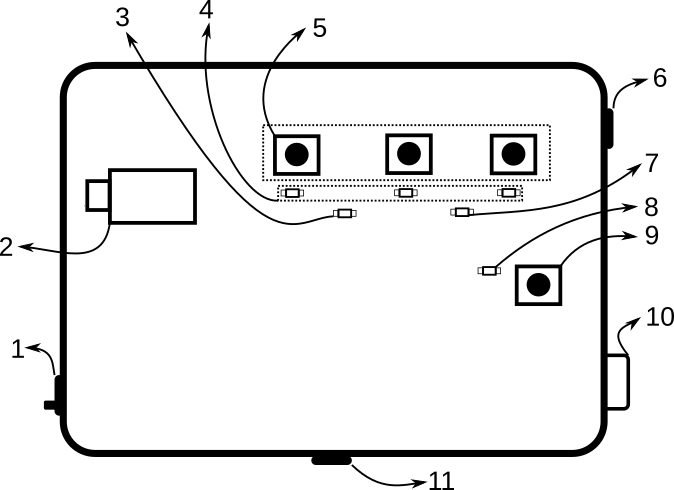
\includegraphics[width=400pt]{part}
		\caption{Layout Dasar Audiometri}
	\end{figure}

	Antarmuka utama audiometri adalah:
	\begin{enumerate}
		\item Jack Audio untuk output nada murni
		\item 3 Lampu indikator untuk 3-Force Choice
		\item 3 Tombol untuk input 3-Force Choice
		\item LED Merah indikator jawaban salah
		\item LED Hijau indikator jawaban benar
		\item LED Biru indikator mode yang sedang berjalan
	\end{enumerate}

	\noindent\makebox[\linewidth]{\rule{\paperwidth}{0.4pt}}\\

	\textbf{Poin klaim:}

	Poin utama paten adalah: Kesederhanaan (\textit{Simplicity}). 
	Simplicity disini ditandai oleh 2 poin:

	\begin{itemize}
		\item Ukuran unit yang portable dan handheld, 110mm X 85mm
		\item Antar Muka ke penggunaa yang sedikit, hanya 3 tombol dan 6 LED.			
	\end{itemize}

	\noindent\makebox[\linewidth]{\rule{\paperwidth}{0.4pt}}\\
	
	Antarmuka tombol dan LED disini memiliki 2 fungsi sekaligus:
	\begin{itemize}
		\item Untuk memulai proses Audiometri dengan urutan tombol agar proses sesi tidak dimulai tanpa disengaja
		\item Untuk proses input 3-Force Choice
	\end{itemize}

	\newpage
	Berikut penjelasan urutan memulai proses sesi Audiometri:
	
	\begin{enumerate}
		\item pastikan LED Biru (no. 6 pada gambar) berkedip sekali setiap 1 detik, sedangkan LED lain mati.
		\item Tekan salah satu tombol di grup tombol 3
		\item LED terdekat tombol akan menyala
		\item Tekan tombol lain selain tombol sebelumnya
		\item LED dekat tombol sebelumnya akan mati, sedangkan LED Hijau/Benar (no. 5 pada gambar) menyala.
		\item Tekan tombol selain dua tombol sebelumnya, maka proses Audiometri dimulai.
		\item LED Biru akan berkedip lebih cepat sebagai indikator proses sesi Audiometri sedang berlangsung	
	\end{enumerate}

	\noindent\makebox[\linewidth]{\rule{\paperwidth}{0.4pt}}\\

	Berikut adalah urutan langkah interaksi 3-Force Choice saat proses Audiometri.
	\begin{enumerate}
		\item Pastikan poin berikut telah siap. Jika belum maka reset kembali unit
		dan ulangi kembali langkah startup.
		\begin{enumerate}
			\renewcommand{\theenumi}{\Alph{enumi}}
			
			\item LED Indikator pada posisi 6 berkedip cepat.
			\item Headphone telah terpasang.
		\end{enumerate}
		
		\item \textbf{Perhatikan} output dari unit.
		\begin{enumerate}
			\renewcommand{\theenumi}{\Alph{enumi}}
			
			\item LED pada baris no.2 akan berkedip sekali bergantian
			\item Nada murni pada output no. 1 akan terdengar,
			bersamaan salah satu LED baris no. 2.
		\end{enumerate}
		
		\item Tekan satu tombol pada baris no.3 dimana LED baris 2 menyala bersamaan dengan terdengar nada murni.
		
		\item LED no. 4 akan menyala satu detik sebagai respon jawaban salah.

		\item LED no. 5 akan menyala satu detik sebagai respon jawaban benar.
		
		\item Lanjutkan hingga LED Mode pada nomor 6 kembali berkedip lambat satu kali setiap satu detik, yang menandakan sesi uji Audiometri selesai.
	\end{enumerate}
	
\end{document}
